\section{Benutzer Interface}



Konzepte, die haupts�chlich dazu dienen mit dem Spieler zu interagieren und sehr abh�ngig von seinen Entscheidungen sind.


\subsubsection{Kompass}
%\begin{wrapfigure}{r}{0.4\textwidth}
 % \begin{center}
  %  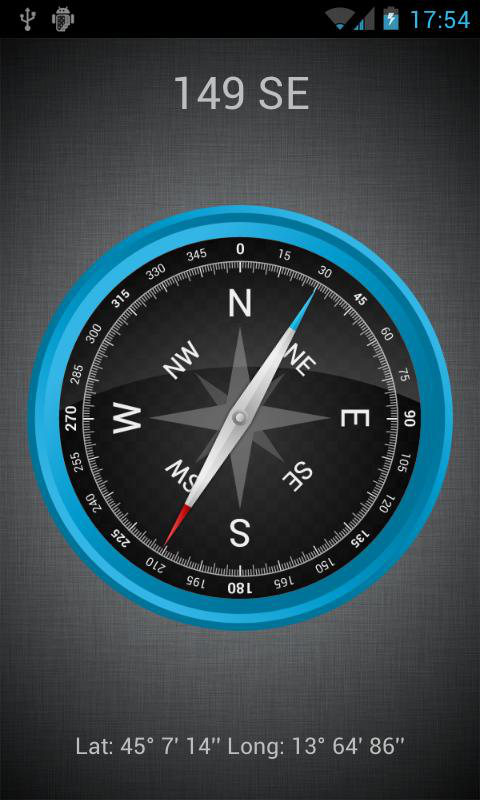
\includegraphics[width=0.3\textwidth]{3-Spielkonzepte/3-2-Benutzer_Interface/kompass.png}
   %  \caption{integrierter Kompass unter Android
	%(Quelle: \url{https://lh6.ggpht.com/tQTY2Itaq9YtG8CZh8RA0N7sekCbURqBG5ZcpV6_u2no8Y8ezVIEibB4udVNFLzYKA\%3Dh900})
%		}
%  \end{center}
%\end{wrapfigure}

Eine Richtungsangabe kann eine Karte ersetzen. Sei es um bei �Capture the Flag� die
Richtung der Fahne des Gegners anzuzeigen oder f�r die �Snake� das n�chste
einzusammelnde Item. In der Regel hat es hier weniger Sinn, wenn die Kompassnadel nach
Norden zeigt.
\newline
Technische L�sungen:
Positionsermittlung (s. \ref{positionsermittlung}), GUI (s. \ref{gui}), Andere Sensorik (s. \ref{sensorik})

\subsubsection{Akustische und haptische Orientierungshilfen}

Akustische oder haptische Signale k�nnen ebenso Hinweise geben auf in der N�he
befindliche Interessengebiete (z.B. ert�nen eines Signals oder Vibration beim Erreichen eines
bestimmtem Umkreises von einem Item). 
Akustische oder haptische Signale k�nnen aber auch als Best�tigung eingesetzt
werden, wenn z.B. etwas eingesammelt wurde.
\newline
Technische L�sungen:
Kollisionsabfrage (s. \ref{kollisionsabfrage}), Andere Sensorik (s. \ref{sensorik})


\subsubsection{Geschwindigkeitsmessung}
Um das Spielgeschehen besser zu kontrollieren zu k�nnen, kann eine Messung der
Geschwindigkeit von Vorteil sein. M�chten wir z.B. bei Capute the Flag dem Fahnentr�ger
nicht erlauben eine gewissen Geschwindigkeit zu �berschreiten, ist eine
Geschwindigkeitsmessung unabdingbar.
\newline
Technische L�sungen:
Positionsermittlung (s. \ref{positionsermittlung}), Server-Client-Kommunikation (s. \ref{kommunikation}), Andere Sensorik (s. \ref{sensorik})


\subsubsection{Mensch-Maschine-Kommunikation}\label{sec:mensch-maschine-kommunikation}
Das komplette Spielgeschehen lebt nach der Integrierung von mobilen Endger�ten von der Kommunikation zwischen Mensch und Ger�t. Wird auf dem Endger�t ein Kompass angezeigt, muss der Spieler insofern reagieren, dass er sich in die richtige Richtung dreht.
Wenn er etwas einsammeln m�chte, kann es erforderlich sein, dass ein Button gedr�ckt
wird.
\newline
Technische L�sungen:
GUI (s. \ref{gui}), Kartendarstellung (s. \ref{kartendarstellung})
